\subsection{\iWildCam}\label{sec:app_iwildcam}

Animal populations have declined 68\% on average since 1970 \citep{grooten_peterson_almond}.
To better understand and monitor wildlife biodiversity loss, ecologists commonly deploy camera traps---heat or motion-activated static cameras placed in the wild \citep{wearn2017camera}---and then use ML models to process the data collected \citep{weinstein2018computer,norouzzadeh2019deep,tabak2019machine,beery2019efficient,ahumada2020wildlife}.
Typically, these models would be trained on photos from some existing camera traps and then used across new camera trap deployments.
However, across different camera traps, there is drastic variation in illumination, color, camera angle, background, vegetation, and relative animal frequencies,
which results in models generalizing poorly to new camera trap deployments \citep{beery2018recognition}.

We study this shift on a variant of the iWildCam 2020 dataset \citep{beery2020iwildcam}.

\subsubsection{Setup}
\paragraph{Problem setting.}
We consider the domain generalization setting, where the domains are camera traps, and we seek to learn models that generalize to photos taken from new camera deployments (\reffig{dataset_iwildcam}).
The task is multi-class species classification.
Concretely, the input $x$ is a photo taken by a camera trap,
the label $y$ is one of 182 different animal species,
and the domain $d$ is an integer that identifies the camera trap that took the photo.

\paragraph{Data.}
The dataset comprises 203,029 images from 323 different camera traps spread across multiple countries in different parts of the world. The original camera trap data comes from the Wildlife Conservation Society (\url{http://lila.science/datasets/wcscameratraps}).
These images tend to be taken in short bursts following motion-activation of a camera trap, so the images can be additionally grouped into sequences of images from the same burst, though our baseline models do not exploit this information and our evaluation metric treats each image individually.
Each image is associated with the following metadata: camera trap ID, sequence ID, and datetime.

As is typical for camera trap data, approximately 35\% of the total number of images are empty (i.e., do not contain any animal species); this corresponds to one of the 182 class labels. The ten most common classes across the full dataset are ``empty'' (34\%), ocellated turkey (8\%), great curassow (6\%), impala (4\%), black-fronted duiker (4\%), white-lipped peccary (3\%), Central American agouti (3\%), ocelot (3\%), gray fox (2\%) and cow (2\%).

We note that the labels in this dataset can be somewhat noisy, as is typical of camera trap data. Some ecologists might label all images in a sequence as the same animal (which can result in empty/dark frames being labeled as an animal), whereas other ecologists might try to label it frame-by-frame. This label noise imposes a natural ceiling on model performance, though the label noise is equally present in ID vs.~OOD data.

We split the dataset by randomly partitioning the data by camera traps:
\begin{enumerate}
  \item \textbf{Training:} 129,809 images taken by 243 camera traps.
  \item \textbf{Validation (OOD):} 14,961 images taken by 32 different camera traps.
  \item \textbf{Test (OOD):} 42,791 images taken by 48 different camera traps.
  \item \textbf{Validation (ID):} 7,314 images taken by the same camera traps as the training set, but on different days from the training and test (ID) images.
  \item \textbf{Test (ID):} 8,154 images taken by the same camera traps as the training set, but on different days from the training and validation (ID) images.
\end{enumerate}
The camera traps are randomly distributed across the training, validation (OOD), and test (OOD) sets. The number of examples per location vary widely from 1 to 8494, with a median of 194 images (\reffig{location_dist_iwildcam}).
All images from the same sequence (i.e., all images taken in the same burst) are placed together in the same split. See \refapp{app_iwildcam_details} for more details.



\begin{figure}[tbp]
  \centering
  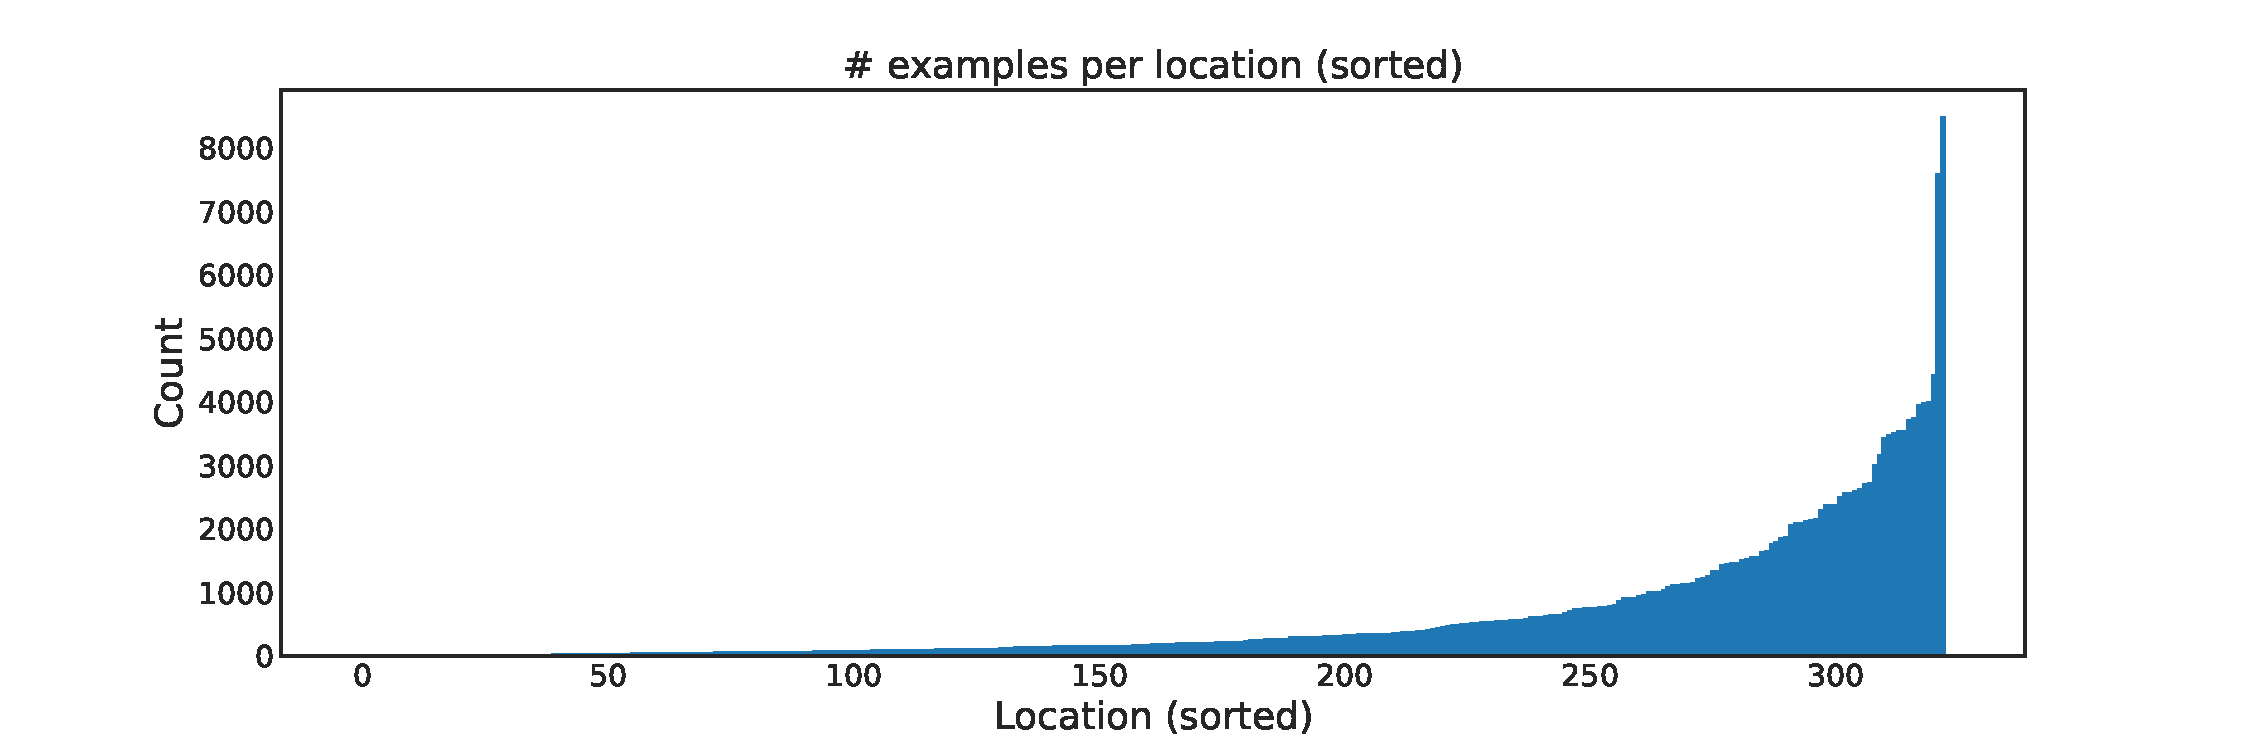
\includegraphics[width=1\linewidth]{figures/iwildcam_location_distribution.pdf}
  \caption{Number of examples per location in the \iWildCam dataset. The locations are sorted such that locations with the least amount of examples are to the left on the x-axis. }\label{fig:location_dist_iwildcam}
\end{figure}

\paragraph{Evaluation.}
We evaluate models by their macro F1 score (i.e., we compute the F1 score for each class separately, then average those scores). We also report the average accuracy of each model across all test images, but primarily use the macro F1 score to better capture model performance on rare species. In the natural world, protected and endangered species are rare by definition, and are often the most important to accurately monitor. However, common species are much more likely to be captured in camera trap images; this imbalance can make metrics like average accuracy an inaccurate picture of model effectiveness.



\paragraph{Potential leverage.} Though the problem is challenging for existing ML algorithms, adapting to photos from different camera traps is simple and intuitive for humans. Repeated backgrounds and habitual animals, which cause each sensor to have a unique class distribution, provide a strong implicit signal across data from any one location.
We anticipate that approaches that utilize the provided camera trap annotations can learn to factor out these common features and avoid learning spurious correlations between particular backgrounds and animal species.

\subsubsection{Baseline results}

\begin{figure*}[tbp]
  \centering
  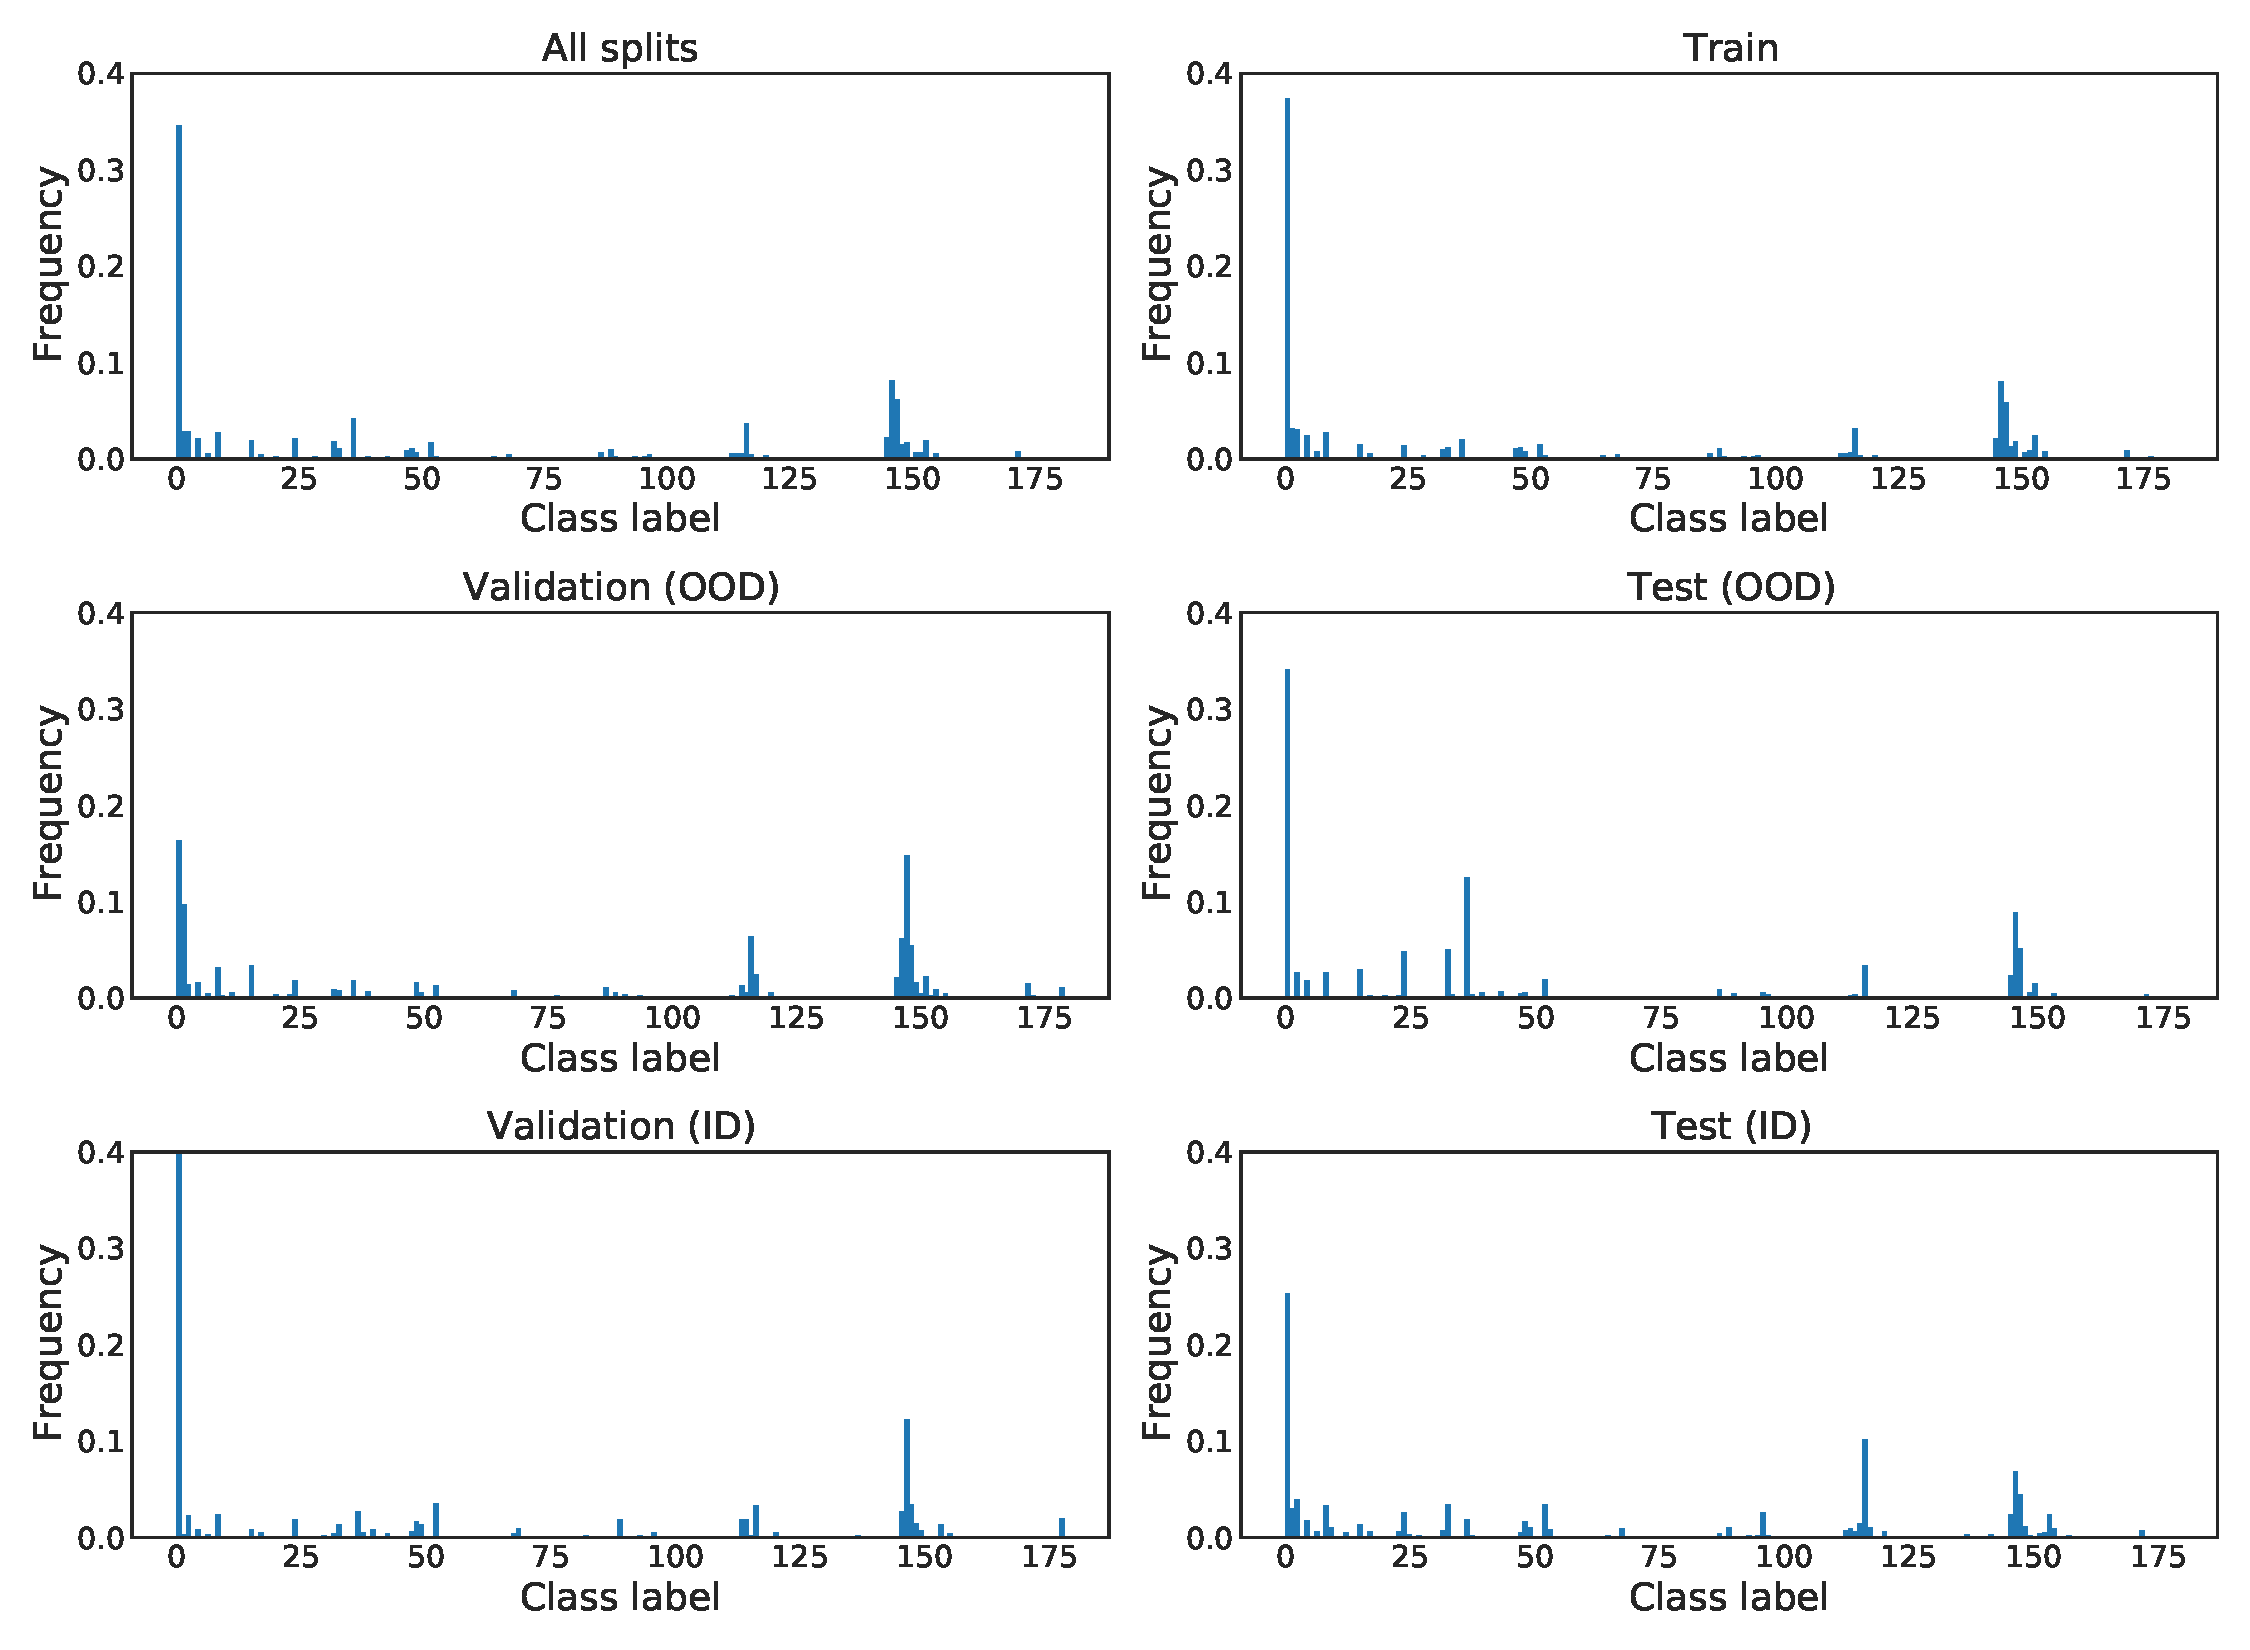
\includegraphics[width=0.9\textwidth]{figures/iwildcam_label_distribution.pdf}
  \caption{Label distribution for each \iWildCam split. }\label{fig:label_dist_iwildcam}
\end{figure*}

\paragraph{Model.} For all experiments, we use ResNet-50 models \citep{he2016resnet} that were pretrained on ImageNet,
using a learning rate of 3e-5 and no $L_2$-regularization.
As input, these models take in images resized to 448 by 448.
We trained these models with the Adam optimizer and a batch size of 16 for 12 epochs. To pick hyperparameters, we did a grid search over learning rates $\{ 1 \times 10^{-5}, 3 \times 10^{-5}, 1 \times 10^{-4}\}$ and $L_2$ regularization strengths $\{ 0,  1 \times 10^{-3}, 1 \times 10^{-2} \}$.
We report results aggregated over 3 random seeds.

\paragraph{ERM results and performance drops.}
Model performance dropped substantially and consistently going from the train-to-train in-distribution (ID) setting to the official out-of-distribution (OOD) setting (\reftab{results_iwildcam}),
with a macro F1 score of 47.0 on the ID test set but only 31.0 on the OOD test set.
We note that macro F1 and average accuracy both differ between the OOD validation and test sets: this is in part due to the difference in class balance between them, which in turn is due to differences in the proportion of classes across camera traps.
In particular, macro F1 can vary between splits because we take the average F1 score across all classes that are present in the evaluation split, and not all splits have the same classes present (e.g., a rare species might be in the OOD validation set but not OOD test set, or vice versa). In additional, average accuracy can differ between splits due in part to variation in the fraction of empty images per location (e.g., the camera traps that were randomly assigned to the OOD validation set have a smaller proportion of empty images).

We only ran a train-to-train comparison because there are a relatively large number of domains (camera traps) split i.i.d.~between the training and test sets, which suggests that the training and test sets should be ``equally difficult''. The size of the ID-OOD gap in macro F1 is large enough that we expect it should hold up even in a test-to-test comparison.
However, the results in \reftab{results_iwildcam} and \reffig{label_dist_iwildcam} show that there is substantial variability between domains, and it would be useful for future work to establish the magnitude of the ID-OOD gap under the test-to-test or mixed-to-test comparisons.

\paragraph{Additional baseline methods.}
\begin{table*}[tbp]
  \caption{Baseline results on \iWildCam. In-distribution (ID) results correspond to the train-to-train setting. Parentheses show standard deviation across 3 replicates.}\label{tab:results_iwildcam}
  \centering
  \resizebox{\textwidth}{!}{\begin{tabular} {l c c c c c c c c}
  \toprule
   & \multicolumn{2}{c}{Val (ID)} & \multicolumn{2}{c}{Val (OOD)} & \multicolumn{2}{c}{Test (ID)} & \multicolumn{2}{c}{Test (OOD)} \\
  Algorithm & Macro F1 & Avg acc & Macro F1 & Avg acc &  Macro F1 & Avg acc & Macro F1 & Avg acc \\
  \midrule
    ERM & 48.8 (2.5) & 82.5 (0.8) & 37.4 (1.7) & 62.7 (2.4) & \textbf{47.0} (1.4) & \textbf{75.7} (0.3) & 31.0 (1.3) & 71.6 (2.5) \\
    CORAL & 46.7 (2.8) & 81.8 (0.4) & 37.0 (1.2) & 60.3 (2.8) & 43.5 (3.5) & 73.7 (0.4) & \textbf{32.8} (0.1) & \textbf{73.3} (4.3)  \\
    IRM & 24.4 (8.4) & 66.9 (9.4) & 20.2 (7.6) & 47.2 (9.8) & 22.4 (7.7) & 59.9 (8.1) & 15.1 (4.9) & 59.8 (3.7) \\
    Group DRO & 42.3 (2.1) & 79.3 (3.9) & 26.3 (0.2) & 60.0 (0.7) & 37.5 (1.7) & 71.6 (2.7) & 23.9 (2.1) & 72.7 (2.0) \\
    Reweighted (label) & 42.5 (0.5) & 77.5 (1.6) & 30.9 (0.3) & 57.8 (2.8) & 42.2 (1.4) & 70.8 (1.5) & 26.2 (1.4) & 68.8 (1.6) \\
  \bottomrule
  \end{tabular}}
\end{table*}
We trained models with CORAL, IRM, and Group DRO, treating each camera trap as a domain, and using the same model hyperparameters as ERM.
These did not improve upon the ERM baseline (\reftab{results_iwildcam}).
The IRM models performed especially poorly on this dataset; we suspect that this is because the default estimator of the IRM penalty term can be negatively biased when examples are sampled without replacement from small domains, but further investigation is needed.
We also tried reweighting the training data so that each label had equal weight, but this did not improve over ERM either. 

\paragraph{Discussion.}
Across locations, there is drastic variation in illumination, camera angle, background, vegetation, and color. This variation, coupled with considerable differences in the distribution of animals between camera traps, likely encourages the model to overfit to specific animal species appearing in specific locations, which may account for the performance drop.

The original iWildCam 2020 competition allows users to use MegaDetector \citep{beery2019efficient}, which is an animal detector trained on a large set of data beyond what is provided in the training set.
Using an animal detection model like MegaDetector typically improves classification performance on camera traps \citep{beery2018recognition}.
However, we intentionally do not use MegaDetector in our baselines for \iWildCam for two reasons.
First, though the trained MegaDetector model is publicly available, the MegaDetector training set is not, which makes it difficult to build on top of it and run controlled experiments.
Second, bounding box annotations are costly and harder to obtain, and there is much more data with image-level species label, so it would be useful to be able to train models that do not have to rely on bounding box annotations.

We still welcome leaderboard submissions that use MegaDetector, as it is useful to see how much better models can perform when they use MegaDetector or other similar animal detectors, but we will distinguish these submissions from others that only use what is provided in the training set.

A different source of leverage comes from the temporal signal in the camera trap images, which are organized into sequences that each correspond to a burst of images from a single motion trigger.
Using this sequence information (e.g., by taking the median prediction across a sequence) can also improve model performance \citep{beery2018recognition},
and we welcome submissions that explore this direction.

\subsubsection{Broader context}
Differences across data distributions at different sensor locations is a common challenge in automated wildlife monitoring applications, including using audio sensors to monitor animals that are easier heard than seen such as primates, birds, and marine mammals \citep{crunchant2020listening, stowell2019automatic, shiu2020deep}, and using static sonar to count fish underwater to help maintain sustainable fishing industries \citep{pipal2012estimating, vatnehol2018method, schneider2020counting}.
As with camera traps, each static audio sensor has a specific species distribution as well as a sensor specific background noise signature, making generalization to new sensors challenging. Similarly, static sonar used to measure fish escapement have sensor-specific background reflectance based on the shape of the river bottom.
Moreover, since species are distributed in a non-uniform and long-tailed fashion across the globe, it is incredibly challenging to collect sufficient samples for rare species to escape the low-data regime.
Implicitly representing camera-specific distributions and background features in per-camera memory banks and extracting relevant information from these via attention has been shown to help overcome some of these challenges for static cameras \citep{beery2020context}.

More broadly, shifts in background, image illumination and viewpoint have been studied in computer vision research. First, several works have shown that object classifiers often rely on the background rather than the object to make its classification \citep{rosenfeld2018elephant, shetty2019not, xiao2020noise}. Second, common perturbations such as blurriness or shifts in illumination, tend to reduce performance \citep{dodge2017study, temel2018cure, hendrycks2019benchmarking}.
Finally, shifts in rotation and viewpoint of the object has been shown to degrade performance \citep{barbu2019objectnet}.


\subsubsection{Additional details}\label{sec:app_iwildcam_details}
\paragraph{Data processing.}
We generate the data splits in three steps. First, to generate the OOD splits, we randomly split all locations into three groups: Validation (OOD), Test (OOD), and Others. Then, to generate the train-to-train ID splits, we split the Others group uniformly by date at random into three sets: Training, Validation (ID), and Test (ID).

When doing the ID split, some locations only ended up in some of but not all of Training, Validation (ID), and Test (ID). For instance, if there were very few dates for a specific location (camera trap), it may be that no examples from that location ended up in the train split. This defeats the purpose of the ID split, which is to test performance on locations that were seen during training. We therefore put these locations in the train split. Finally, any images in the test set with classes not present in the train set were  removed.

\paragraph{Modifications to the original dataset.}
The original iWildCam 2020 Kaggle competition similarly split the dataset by camera trap, though the competition focused on average accuracy. We consider a smaller subset of the data here.
Specifically, the Kaggle competition uses a held-out test set that we are not utilizing, as the test set is intended to be reused in a future competition and is not yet public.
Instead, we constructed our own test set by splitting the Kaggle competition training data into our own splits: train, validation (ID), validation (OOD), test (ID), test (OOD).

Images are organized into sequences, but we treat each image separately. In the iWildCam 2020 competition, the top participants utilized the sequence data and also used a pretrained MegaDetector animal detection model that outputs bounding boxes over the animals. These images are cropped using the bounding boxes and then fed into a classification network. As we discuss above, we intentionally do not use MegaDetector in our experiments.

In addition, compared to the iWildCam 2020 competition, the iWildCam 2021 competition changed several class definitions (such as removing the ``unknown'' class) and removed some images that were taken indoors or had humans in the background. We have applied these updates to \iWildCam as well.
